%%%%%%%%%%%%%%%%%%%%%%%%%%%%%%%%%%%%%%%%%%%%%%%%%%%%%%%%%%%%%%%%%%%%%%%%%%%%%%%%
%2345678901234567890123456789012345678901234567890123456789012345678901234567890
%        1         2         3         4         5         6         7         8

\documentclass[letterpaper, 10 pt, conference]{ieeeconf}  % Comment this line out if you need a4paper

%\documentclass[a4paper, 10pt, conference]{ieeeconf}      % Use this line for a4 paper

\IEEEoverridecommandlockouts                              % This command is only needed if 
                                                          % you want to use the \thanks command

\overrideIEEEmargins                                      % Needed to meet printer requirements.
\usepackage{cite}
\usepackage{amsmath,amssymb,amsfonts}
\usepackage{graphicx}
\usepackage{textcomp}
\usepackage{xcolor}
\usepackage{bm}
\usepackage{float}
\usepackage{subcaption}

\usepackage[ruled]{algorithm2e}
\SetKwComment{Comment}{$\triangleright$ }{}
\usepackage{tabu}
\usepackage{booktabs}
\usepackage{etoolbox}
\usepackage{hyperref}
\usepackage{todonotes}
\usepackage{svg}
\def\BibTeX{{\rm B\kern-.05em{\sc i\kern-.025em b}\kern-.08em
		T\kern-.1667em\lower.7ex\hbox{E}\kern-.125emX}}
\graphicspath{ {images/} }

%In case you encounter the following error:
%Error 1010 The PDF file may be corrupt (unable to open PDF file) OR
%Error 1000 An error occurred while parsing a contents stream. Unable to analyze the PDF file.
%This is a known problem with pdfLaTeX conversion filter. The file cannot be opened with acrobat reader
%Please use one of the alternatives below to circumvent this error by uncommenting one or the other
%\pdfobjcompresslevel=0
%\pdfminorversion=4

% See the \addtolength command later in the file to balance the column lengths
% on the last page of the document

% The following packages can be found on http:\\www.ctan.org
%\usepackage{graphics} % for pdf, bitmapped graphics files
%\usepackage{epsfig} % for postscript graphics files
%\usepackage{mathptmx} % assumes new font selection scheme installed
%\usepackage{times} % assumes new font selection scheme installed
%\usepackage{amsmath} % assumes amsmath package installed
%\usepackage{amssymb}  % assumes amsmath package installed

\title{\LARGE \bf
	Learning to Fail: Failure Plans and Predictions for Crowd Navigation
}


\author{Patrick Naughton$^{1}$, Ishani Chatterjee$^{2}$, Tushar Kusnur$^{3}$, and Maxim Likhachev$^{4}$% <-this % stops a space
\thanks{Some text}% <-this % stops a space
\thanks{$^{1}$Notes
        {\tt\small patrickrnaughton@wustl.edu}}%
\thanks{$^{2}$Ishani notes
        {\tt\small ichatter@andrew.cmu.edu}}%
}


\begin{document}



\maketitle
\thispagestyle{empty}
\pagestyle{empty}


%%%%%%%%%%%%%%%%%%%%%%%%%%%%%%%%%%%%%%%%%%%%%%%%%%%%%%%%%%%%%%%%%%%%%%%%%%%%%%%%
\begin{abstract}
	When navigating in the presence of humans, mobile robots need robust, efficient ways of dealing with highly stochastic dynamic obstacles. This problem is often addressed by building a (implicit or explicit) model of possible human trajectories and planning the robot's motion based on this model to avoid collisions. We call this a \textit{success controller}. However, such controllers typically assume that their goal is feasible, without considering cases in which humans may move to block the robot's path. This can lead to the robot simply stopping, continuously replanning to an infeasible goal, or, in the worst case, colliding with a pedestrian. This work seeks to explicitly address this deficiency by creating a classifier that examines the robot's trajectory to determine whether or not it believes the robot can efficiently achieve its goal point. Additionally, we develop a \textit{failure controller} that the robot executes if the classifier determines that it cannot reach its goal. This controller safely guides the robot to a different location from which it can replan. We show that this failure controller results in fewer intrusions near people in a crowded scene than simply relying on the success controller.
\end{abstract}


%%%%%%%%%%%%%%%%%%%%%%%%%%%%%%%%%%%%%%%%%%%%%%%%%%%%%%%%%%%%%%%%%%%%%%%%%%%%%%%%
\section{INTRODUCTION}

	The contributions of this work are:
	\begin{enumerate}
		\item A classifier that determines whether or not a robot is likely to reach its goal in a given scene.
		\item A failure controller that safely guides the robot to a stable position from which it can initiate replanning.
	\end{enumerate}
	

\section{RELATED WORK}
	Several methods use explicit models of human behavior to achieve smooth, predictable robot navigation among pedestrians. Trautman et al. model the interaction between the robot and pedestrians as an extension of an interactive Gaussian process that accommodates multiple goals \cite{caseforcoop}. The social forces model treats humans and the robot in question as masses subject to Newtonian dynamics and applies fictitious forces to them to predict and plan trajectories \cite{sfm}. It recomputes these forces and their effects on robot motion at each time step to determine how the robot should move. These techniques however rely on hand-crafted models of human behavior to achieve their results and handle unexpected or uncooperative human actions by simply replanning using the same model. The social forces model in particular does not demonstrate robust navigation plans and will sometimes exhibit oscillatory behavior in more crowded or narrow areas \cite{sfm}.
	
	Another approach uses inverse reinforcement learning to learn latent, possibly stochastic social rules humans observe when navigating in crowds \cite{socialirl}. This method uses example trajectories recorded from humans or gathered from teleoperated runs. This approach however is extremely unlikely to observe failed trajectories where a human attempts to execute some navigation plan and is forced to completely abort their initial goal. If a human attempts to overtake someone else, for example, they have many contingency options in the case where the other person is either intentionally or unintentionally uncooperative. For example, they could use verbal communication or body language to more explicitly communicate their intentions, options which are not available to many mobile robots. For this reason, inverse reinforcement learning will likely be unable to formulate a useful model for navigation when situations such as these occur.
	
	Reinforcement learning has successfully been applied to the social robot navigation problem using a variety of different models \cite{sociallyawarerl}, \cite{crowdawarerl}. Reinforcement learning is particularly suited to this application as noted in \cite{sociallyawarerl} because it is extremely difficult to specify what the optimal action for a robot to take is, but it is comparatively easy to alert the robot when it performs a socially unacceptable or unsafe action. Previous work has focused on using reinforcement learning to develop policies that generate optimal (in terms of time) paths to a robot's goal in the presence of humans or other autonomous agents. These policies however generally assume the goal is reachable and do not make contingency plans if that assumption turns out to be incorrect. Additionally, the agent is explicitly given a goal to reach by the experimenters; we wish to navigate in the case of failure at which point there is no obvious goal.
	
	The above methods all either deal with failure at execution time by simply replanning or do not consider failure to reach the goal at all. We depart from this paradigm by designing a controller specifically targeted at producing trajectories when the robot's original goal is no longer reachable.
	
\section{PROBLEM STATEMENT}
	We consider a robot that strings together different motion primitives and controllers to generate a navigation policy to reach some overall goal. Motion primitives are basic actions the robot can take which are guaranteed to succeed, for example, drive forward one meter. Controllers are more complicated actions that may fail, for example, barging past a group of pedestrians. These controllers can be used by the robot in specific situations to navigate in a scene. We refer to the controller that guides the robot a \textit{success controller}. This work is concerned with detecting and handling the failure of these controllers. Specifically, we develop a \textit{failure controller} that corresponds to a given success controller. This failure controller directs the robot if it is determined at execution time that the success controller is unlikely to achieve its goal. 
	
	Additionally, we would like to rigorously determine at execution time whether or not the success controller is likely to succeed. In this framework, the robot can decide at each time step whether it should begin using the failure controller. Once it switches to the failure controller, it cannot switch back to the success controller until the planner generates a new plan. 
		
\section{APPROACH}
	We begin with a fixed success controller. In this work, we consider one specific controller for barging into a group of people at the end of a corridor. While the experiments and results here only concern this controller, the framework can be extended to include other controllers as well, for example, to overtake or cross in front of pedestrians. In order to train this controller, we first generate example runs in which the robot can reach its goal using the RVO2 simulator \cite{rvo2}, \cite{pyrvo2}. We employ a neural network architecture based on the one presented in \cite{crowdawarerl} to allow the network to handle variable input sizes. The state of the robot is characterized by ... In addition, we include an LSTM at the end of our network so that the robot can learn the sequence of actions. Figure \ref{fig:model_arch} shows the overall architecture of the network. The output of the network has five nodes which are interpreted as the $x$ and $y$ coordinates of the mean, the $x$ and $y$ standard deviations, and the correlation between $x$ and $y$ of a Gaussian distribution of the next location of the robot conditioned on its current state. At execution time, we then feed this network its current state and attempt to move to the mean of this distribution in the next time step.
	
	\begin{figure}
		\centering
		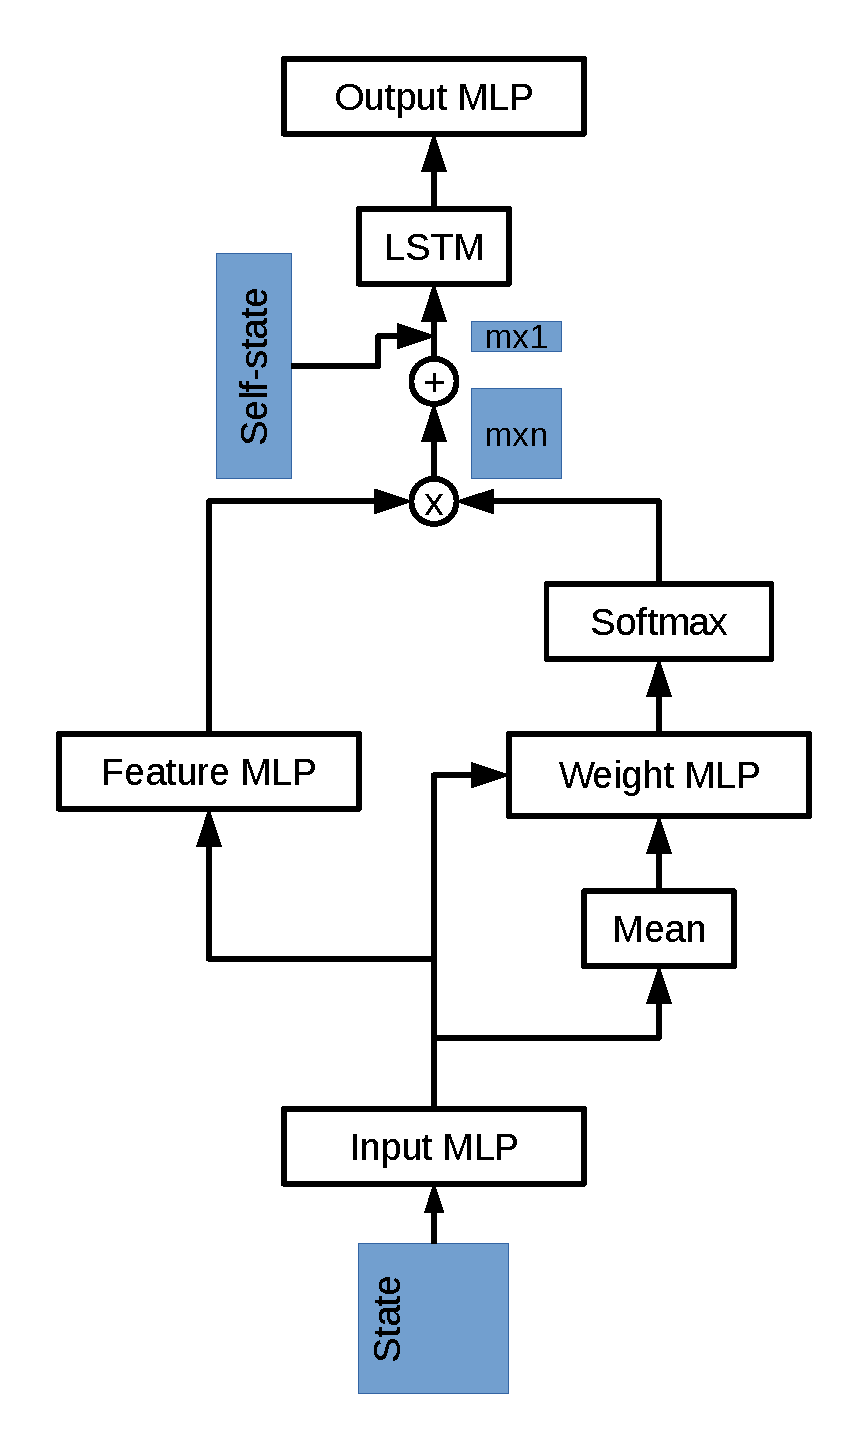
\includegraphics[height=\linewidth, angle=270]{model_arch.pdf}
		\caption{Model architecture}
		\label{fig:model_arch}
	\end{figure}
	
	We split the approach into two distinct parts: First, we consider just determining whether or not the robot should switch to its failure controller. Given this classifier, we then develop a failure controller that, starting from the state at which the classifier reports we have failed, attempts to learn a policy that guides the robot to a safe location from which to replan.
	
	\subsection{Determining When To Switch}
		In order to rigorously determine whether or not the success controller is likely to succeed (and thus, whether or not we should switch to the failure controller), we train an additional neural network that has the same architecture as the original. However, it attempts to learn a target function that predicts the distribution of previous locations of the robot given the robot's current state and the fact that the robot is on a trajectory that leads to its goal. It is trained on trajectories generated by the success controller in scenes where the success controller can reach its goal. This network however does not receive the robot's full state, rather, it only observes the robot's \textit{self state}, that is, its ... This was done so that we could train the network by only showing it successful trajectories without the uncertainty in its prediction exploding when it observes unsuccessful ones. 
		
		At execution time, we utilize this network's prediction to perform a statistical $p$-test with an $\alpha$ value of $0.02$. At each time step we construct the error ellipse given by the Gaussian distribution represented by the reverse predictor that contains $1-\alpha$ of the distribution's probability mass. By default, we assume that the trajectory will be successful and switch to the failure controller only if the robot's previous position falls outside the predicted error ellipse.
	
	\subsection{Failure Controller}
		For the failure controller, we need to address a somewhat novel formulation of the navigation problem in that the robot now has no specific goal it is trying to reach. Once the failure controller gets invoked, the robot has determined that it is unlikely to reach its goal. Because it is impossible to explicitly define optimality in this framework, we formulate this as a reinforcement learning problem and model the robot as a Markovian agent. Rather than define a set of states constituting a goal, we define a reward function that punishes actions we determine to be undesirable. 
		
		Our reward function is split into three parts: $\mathcal{R}_{\text{collision}}$, $\mathcal{R}_{\text{movement}}$, and $\mathcal{R}_{\text{smoothness}}$. The overall reward the robot observes is simply the sum of these three components. Equations 
		
		\begin{equation}
			\mathcal{R}_{\text{collision}} = \begin{cases}
				-1      &   d < 0\\
				-0.25   &   0 \leq d < 0.2\\
				0       &   else
			\end{cases}
		\end{equation}
		
		\begin{equation}
			\mathcal{R}_{\text{movement}} = \begin{cases}
			0       &   a_t = 0 \quad(remain\;still)\\
			-0.01   &   else
			\end{cases}
		\end{equation}
		
		\begin{equation}
			\mathcal{R}_{\text{smoothness}} = \begin{cases}
			0       &   a_t = a_{t-1} \vee a_{t-1} = 0\\
			-0.01   &   else
			\end{cases}
		\end{equation}

\section{RESULTS}

\section{CONCLUSIONS}



%\addtolength{\textheight}{-12cm}   % This command serves to balance the column lengths
                                  % on the last page of the document manually. It shortens
                                  % the textheight of the last page by a suitable amount.
                                  % This command does not take effect until the next page
                                  % so it should come on the page before the last. Make
                                  % sure that you do not shorten the textheight too much.

%%%%%%%%%%%%%%%%%%%%%%%%%%%%%%%%%%%%%%%%%%%%%%%%%%%%%%%%%%%%%%%%%%%%%%%%%%%%%%%%



%%%%%%%%%%%%%%%%%%%%%%%%%%%%%%%%%%%%%%%%%%%%%%%%%%%%%%%%%%%%%%%%%%%%%%%%%%%%%%%%



%%%%%%%%%%%%%%%%%%%%%%%%%%%%%%%%%%%%%%%%%%%%%%%%%%%%%%%%%%%%%%%%%%%%%%%%%%%%%%%%

\section*{ACKNOWLEDGMENT}



%%%%%%%%%%%%%%%%%%%%%%%%%%%%%%%%%%%%%%%%%%%%%%%%%%%%%%%%%%%%%%%%%%%%%%%%%%%%%%%%

\bibliographystyle{IEEEtran}
\bibliography{ref}

\end{document}
